\documentclass{article}
\usepackage[utf8]{inputenc}
\usepackage{graphicx}
\usepackage[margin=0.5in]{geometry}
\title{Stat490 Homework}
\author{ANDY LI}
\date{February 2023}

\begin{document}
\maketitle
We want MSTr and MSE.
$E(SSTr) = E[\sum_{j=1}^vn_j(A_j-\mu)^2] \Rightarrow$
\\
$E(SSTr) = \sum_{j=1}^vn_j(A_j-\mu)^2 \Rightarrow$
\\
$E(SSTr) = \sum_{j=1}^vn_jVar(A_j) \Rightarrow$
\\
$E(SSTr) = va^2_A$
\\
$E(MSTr) = E[\frac{SSTr}{df_{Treatment}}] \Rightarrow$
\\
$E(MSTr) = \frac{va^2_A}{v-1}$
\\v is the number of treatments.
\\
$E(SSE) = E[\sum_{i=1}^k\sum_{j=1}^n(x_{ij}-A_i-B_j)^2] \Rightarrow$
\\
$E(SSE) = \sum_{i=1}^k\sum_{j=1}^n(x_{ij}-A_i-B_j)^2 \Rightarrow$
\\
$E(SSE) = E[\sum_{i=1}^k\sum_{j=1}^nVar(\sum(j)) \Rightarrow$
\\
$E(SSE) = vna^2$ 
\\n is the number of blocks.
\\
$E(MSE) = E[\frac{SSE}{df_{Error}}] \Rightarrow$
\\
$E(MSE) = \frac{vna^2}{(v-1)(n-1)}$
\\
$F = \frac{MSTr}{MSE} \Rightarrow$
\\
$F = \frac{\frac{va^2_A}{v-1}}{\frac{vna^2}{(v-1)(n-1)}} \Rightarrow$
\\
$F = \frac{a^2_A(n-1)}{na^2}$

\section*{4.11}
a)
\\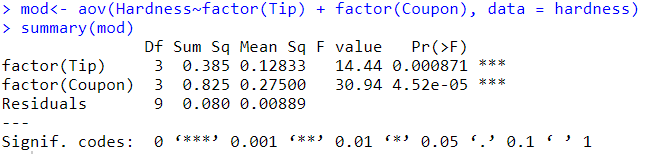
\includegraphics{4.11a.PNG}
\\From the ANOVA table, we get a p value of 0.000871, so we can reject the null hypothesis at the 0.05 significance level. Therefore, there is enough evidence from the data to conclude a difference in means for the 4 Tips.
\\
\\b)
\\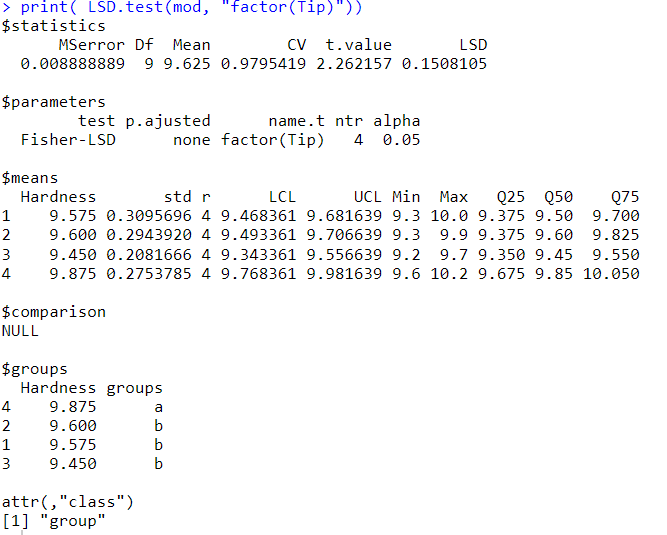
\includegraphics{4.11b.PNG}
\\From the LSD test, we see that Tip 4 has a different mean than Tips 1, 2, and 3.
\\
\\c)
\\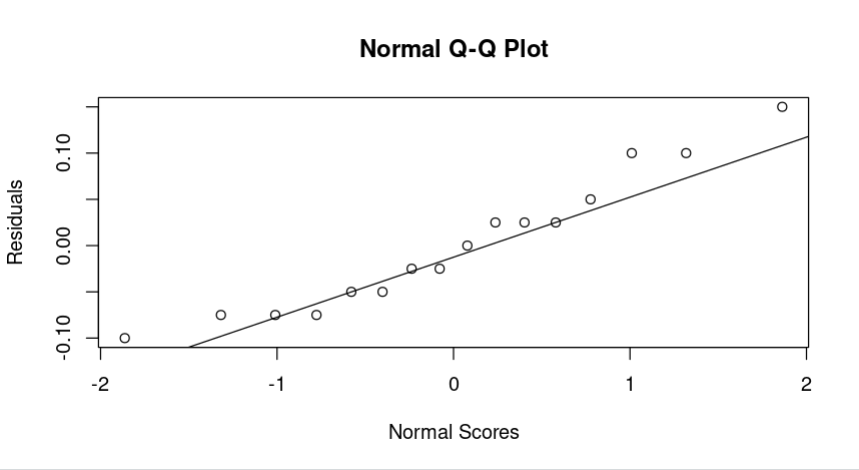
\includegraphics{4.11cQQ.PNG}
\\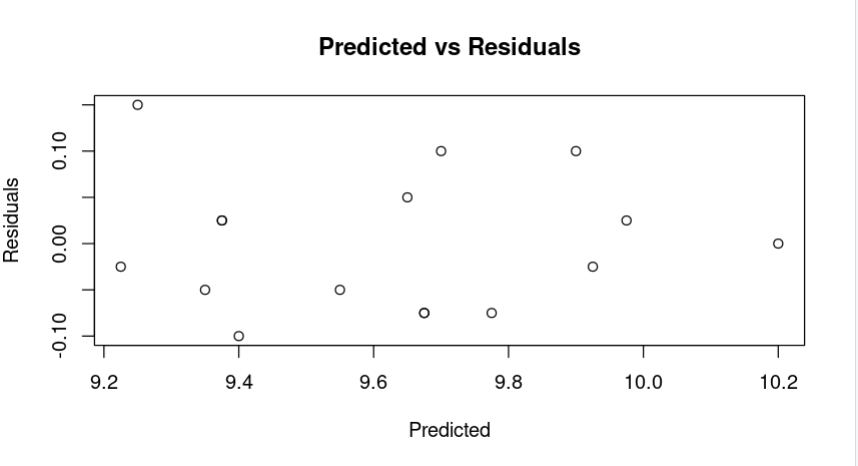
\includegraphics{4.11cRes.PNG}
\\From the residual plots above, we can see that both plots provide evidence for an approximately normal distribution. Residuals are spread evenly.
\newpage
\section*{4.15}
a)
\\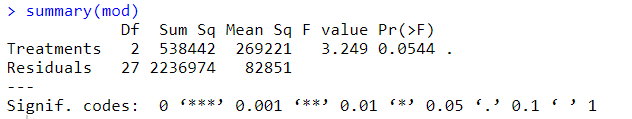
\includegraphics{4.15a.PNG}
\\From the ANOVA table, we see a p value of 0.0544 which tells us to fail to reject the null that there is no difference in treatment means at the 0.05 significance level.
\\
\\b)
\\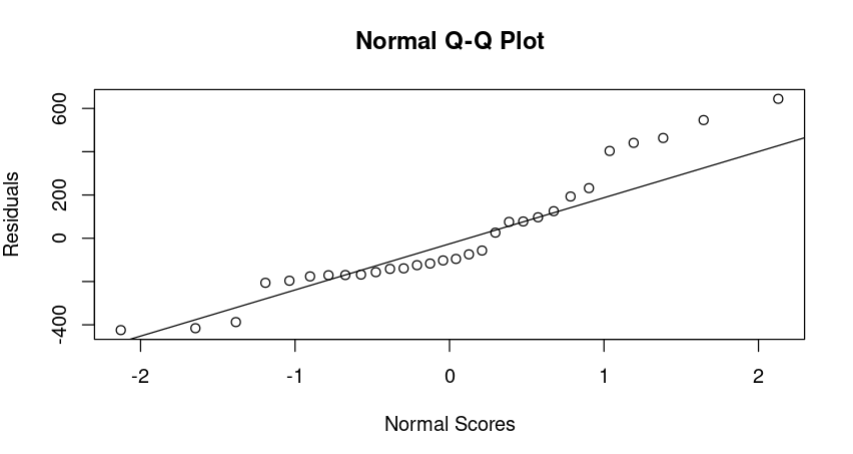
\includegraphics{4.15bQQ.PNG}
\\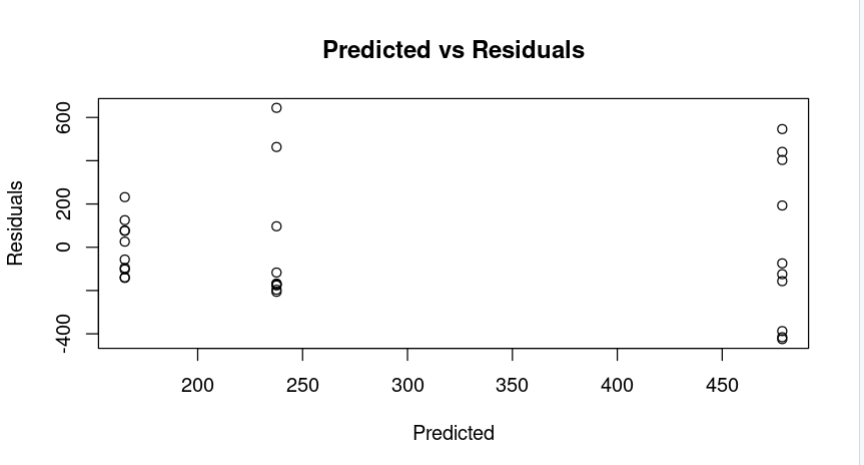
\includegraphics{4.15bRes.PNG}
\\From the residual plots the distribution do not follow a normal distribution
\\
\\c)
\\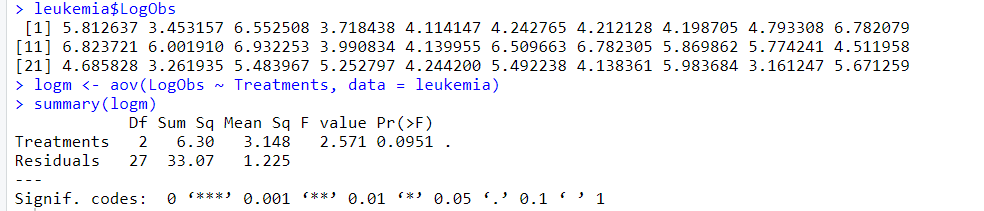
\includegraphics{4.15c.PNG}
\\From the ANOVA table, we see a p value of 0.0951 which tells us to fail to reject the null that there is no difference in log of treatment means at the 0.05 significance level.
\\
\\d)
\\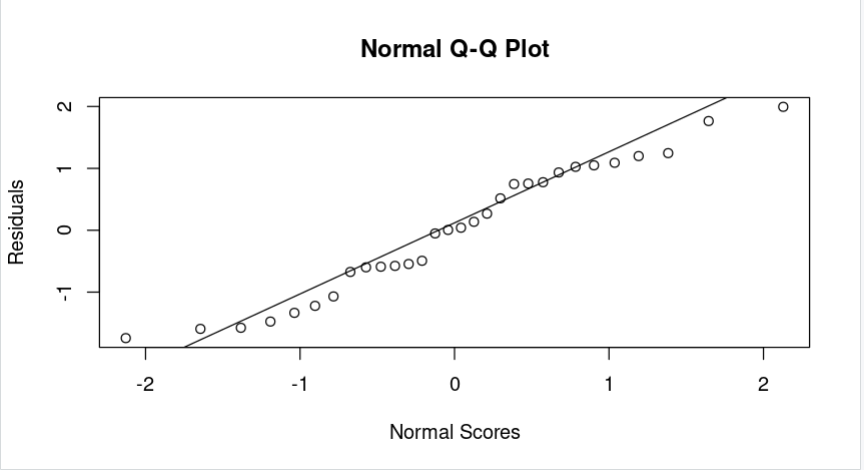
\includegraphics{4.15dQQ.PNG}
\\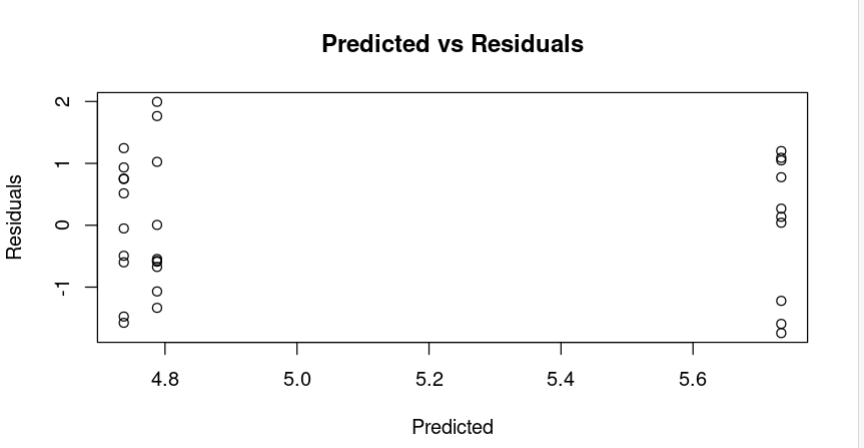
\includegraphics{4.15dRes.PNG}
\\From the transformed residual plots, we see that the data is more normal than untransformed. In the QQ plot, the points roughly follow the linear model, so the transformed distribution is approximately normal.

\section*{4.24}
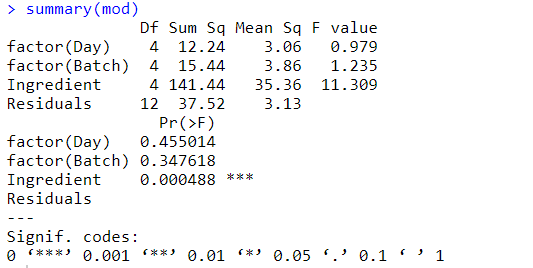
\includegraphics{4.24.PNG}
\\From the ANOVA table, we observe that the Ingredient factor has a p value of 0.000488. Because this p value is smaller than $\alpha = 0.05$, we reject the null hypothesis which says that the means of observations between ingredients are all the same.
\newpage
\section*{4.27}
    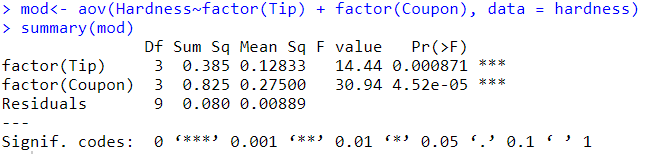
\includegraphics{4.11a.PNG}
    \\Estimate block variance components.
    $$\hat{\sigma}^2 = MSE$$
    $$\hat{\sigma}_B^2 = \frac{(MSBl - MSE)}{a}$$
    \\$\hat{\sigma}^2 = 0.00889$
    \\$\hat{\sigma}_B^2 = 0.066578$

\section*{4.42}
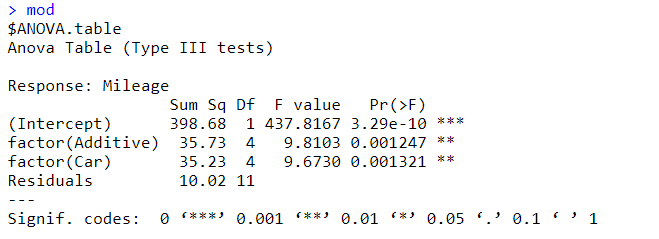
\includegraphics{4.42.PNG}
\\From the BIBD ANOVA table, we see that the gas additive p value is 0.001247 which is less than $\alpha = 0.05$. This means we can reject the null hypothesis which says that the mean mileages for the 5 gas additives are the same.

\section*{4.48}
Given $a = 8$, $b = 14$, $k = 4$, and $\lambda = 3 = \frac{r(k-1)}{a-1} \Rightarrow r = 7$ 
\\$a = 8$, $b = 14$, $\lambda = 3$, $r = 7$, $k = 4$
\\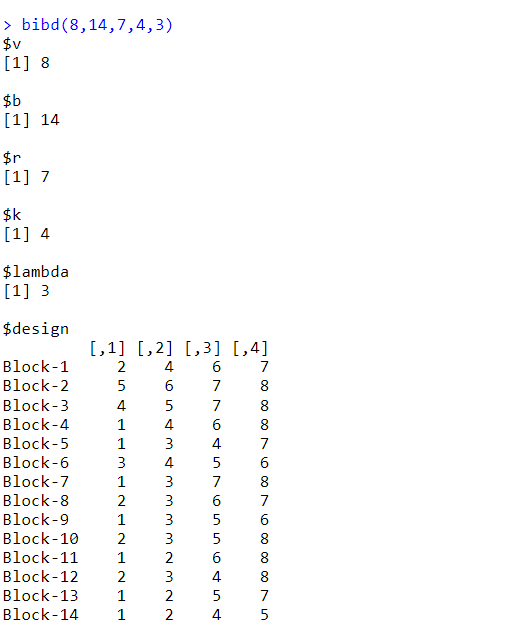
\includegraphics{4.48a.PNG}
\\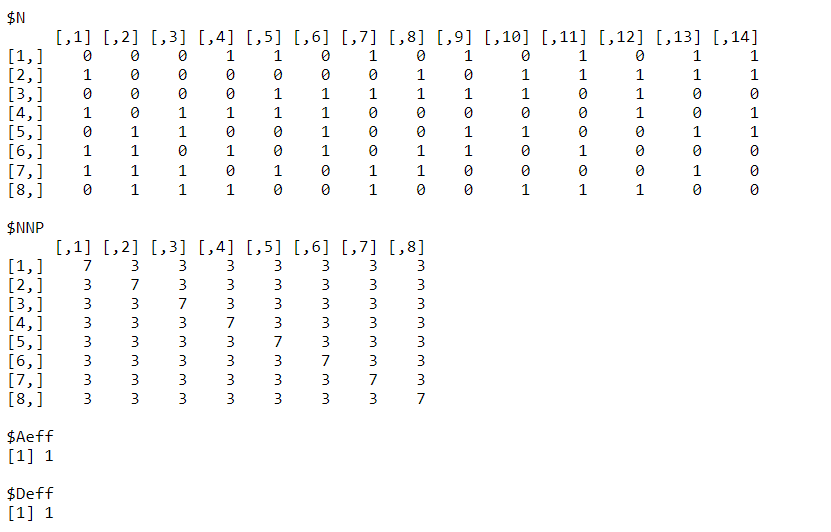
\includegraphics{4.48b.PNG}
\end{document}